\documentclass[master=cws,masteroption=gs]{kulemt}
\setup{title={Schaalbare genoomanalyse met NoSQL- databases},
		author={Brecht Gossel\'e},
		promotor={Prof. Dr. Roel Wuyts},
		assessor={},
		assistant={Prof. Dr. Roel Wuyts}}
\setup{filingcard,
		translatedtitle=,
		udc=,
		shortabstract={Here comes a very short abstract, containing no more than 500 words. \LaTeX\ commands can be used here.}}
		
\usepackage{url}
\usepackage{graphicx}
\usepackage{booktabs}
\graphicspath{ {afbeeldingen/} }
\usepackage{listings}
\usepackage[pdfusetitle,colorlinks,plainpages=false]{hyperref}

\begin{document}

\begin{preface}
\end{preface}

\tableofcontents

\begin{abstract}
\end{abstract}


\mainmatter

\include{inleiding}
\chapter{Achtergrond databanken}
\label{cha2}

Sinds de jaren '70 zijn zogenaamde \textit{relational database management systems} (kortweg RDBMS) de voornaamste technologie voor de grootschalige opslag van gegevens. Ze zijn gestoeld op 2 belangrijke principes, namelijk het relationele datamodel \cite{codd1970relational} en de gestructureerde querytaal SEQUEL, beter gekend als SQL \cite{chamberlin1974sequel}. De architectuur van vele RDBMS is nog steeds gebaseerd op de eerste implementatie van een dergelijk systeem, namelijk het IBM onderzoeksproject System R \cite{blasgen1981system}, ook uit halverwege de jaren '70. System R is uiteraard ontworpen voor destijds relevante hardwarekarakteristieken en productvereisten: business data processing via een command line interface, en dit op computersystemen met trage processoren, kleine werk- en schijfgeheugens maar relatief grote bandbreedte tussen de schijfopslag en het werkgeheugen \cite{Stonebraker:2007:EAE:1325851.1325981}. Dit leidde tot een aantal architecturale features die nog steeds terug te vinden zijn in hedendaagse RDBMS:
\begin{itemize}
\item Disk-geori\"enteerde opslag- en indexstructuren
\item Multithreading om latency te verbergen
\item Concurrency-controlemechanismen op basis van locking
\item Log-gebaseerd herstel van fouten
\end{itemize} 
Ondanks gigantische technologische vooruitgang op gebied van hardware en sterk gediversifieerde gebruiksscenario's, is er sinds hun ontstaan 40 jaar geleden weinig drastisch veranderd aan het concept van de RDBMS en zijn deze systemen de werkpaarden van de industrie geworden op het vlak van dataopslag.\\

Beginnende in de jaren 2000 groeide in de IT-wereld dan ook het besef dat de rigide "one size fits all"-aanpak van RDBMS voor vele moderne toepassingen achterhaald dreigde te geraken. Met grote opkomende spelers uit de <eb-industrie zoals Google, Amazon en Facebook aan het roer leidde dit tot de opkomst van de NoSQL-beweging. NoSQL staat, in tegenstelling tot wat de naam doet vermoeden, voor "Not only SQL" en omvat een waaier van uiteenlopende alternatieve gegevensopslagsystemen die elk in bepaalde specifieke opzichten meerwaarde trachten te bieden ten opzichte van het klassieke relationele systemen. In tegenstelling tot de 'Zwitsers zakmes'-aanpak van RDMBS, leggen ze zich toe op zeer gespecialiseerde toepassingsdomeinen en proberen daarin relationele systemen te overtreffen. Vaak betekent dit dat NoSQL systemen vele voor hun doel onnodig geachte features van SQL systemen achterwege laten, of afzwakken. Een goed voorbeeld hiervan zijn de ACID-eigenschappen uit het relationele model die in vele NoSQL-systemen gereduceerd zijn tot zogenaamde BASE-eigenschappen (op het verschil tussen beide komt onderstaande sectie nog uitgebreid terug).

\section{Begrippen}

Deze sectie belicht de belangrijkste technische begrippen in verband met NoSQL-databanken en contrasteert waar nodig met gelijkaardige concepten in het klassieke traditionele model.

\paragraph{Consistentie}

Consistentie van database-transacties betekent dat transacties de databank in een consistente staat achterlaten: alle data die een applicatie kan zien, is een consistente snapshot van de databank \cite{ports2010transactional}. Traditionele RDBMS bieden vaak transacties met de zogenaamde ACID-eigenschappen \cite{haerder1983principles}:
\begin{itemize}
\item \textbf{Atomicity:} Elke transactie gebeurt ofwel volledig, ofwel helemaal niet.
\item \textbf{Consistency:} Elke transactie laat de databank in consistente staat achter.
\item \textbf{Isolation:} Elke transactie verloopt volledig ge\"isoleerd van elke andere transactie en be\"invloedt deze dus op geen enkele manier.
\item \textbf{Durability:} Eens voltrokken, blijft elke transactie duurzaam bewaard in de databank, ook in het geval van stroomonderbrekingen, crashes of fouten.
\end{itemize}

Zoals Eric Brewer stelde in zijn bekende CAP-theorema \cite{brewer2000towards}, is het in een gedistribueerd systeem niet eenvoudig zowel consistentie, availability als tolerantie voor partities te bereiken en zijn 2 van deze 3 eigenschappen het hoogst haalbare\footnote{Brewer kwam hier zelf 12 jaar later op terug, stellende dat mits goede omgang met partities het toch mogelijk is een trade-off van alle drie te bereiken \cite{brewer2012cap}.}.
Ook in NoSQL-systemen, die vaak gedistribueerd van aard zijn, is het garanderen van consistentie geen triviale opgave. Afhankelijk van de gehanteerde schrijfstrategie is het mogelijk dat verschillende knopen in het cluster verschillende versies van data zien, als updates nog niet in het volledige cluster doorgekomen zijn. Daarom is er het onderscheid tussen strikte en uiteindelijke ("\textit{eventual}") consistentie: strikte consistentie is de gekende vorm waarin updates onmiddellijk zichtbaar zijn op alle nodes in het cluster, en dus ook naar bovenliggende applicaties toe. In het geval van uiteindelijke consistentie garandeert het systeem enkel dat na verloop van tijd alle nodes in het cluster dezelfde, up-to-date versie van de data zullen zien. NoSQL-systemen bieden dan ook vaak de BASE-eigenschappen, een zwakkere versie van de ACID-garanties:
\begin{itemize}
\item \textbf{Basically available:} Het systeem is onder quasi alle omstandigheden beschikbaar.
\item \textbf{Soft state:} Het systeem verkeert niet altijd in een consistente staat
\item \textbf{Eventually consistent:} Na verloop van tijd zal het systeem in een gekende staat verkeren.
\end{itemize}

Vele NoSQL-systemen stellen de gebruiker echter niet voor een voldongen feit bij de keuze tussen strikte en uiteindelijke consistentie: dankzij zogenaamde \textit{quora} kan de gebruiker zelf configureren welke consistentie het systeem levert. Door lees- en schrijfquora in te stellen, kan de gebruiker tunen hoeveel replica's respectievelijk moeten returnen bij een schrijfopdracht, en het welslagen van een schrijfopdracht moeten bevestigen. Op deze manier kan de gebruiker zelf een trade-off maken tussen snel lezen, schrijven en de behaalde consistentie. Bovendien zal de gebruiker, wanneer de som van het lees- en schrijfquorum groter is dan de replicatiefactor van het cluster, steeds de meest recente versie van gegevens zien, wat hetzelfde betekent als onmiddellijke, strikte consistentie.

\section{NoSQL-klassen}

NoSQL databanken zijn er in verschillende soorten en kunnen op basis van hun datamodel in een aantal categorie\"en onderverdeeld worden:

\begin{itemize}
\item \textbf{Key-Value stores} Deze zijn vergelijkbaar met dictionaries en mappen unieke keys op values. Deze values zijn voor de databank volledig betekenisloze byte-arrays en de enige manier om ze op te vragen, is via de bijhoren key. Voor zeer eenvoudige toepassingen resulteert dit in hoge lees- en schrijf-throughput, maar meer geavanceerde features zoals indexing, queries, en het modelleren van relaties binnen de data zijn hierdoor niet mogelijk\cite{hecht2011nosql}\cite{grolinger2013data}.

\item \textbf{Columnar stores} Deze zijn gebaseerd op het datamodel dat Google's BigTable heeft ge\"introduceerd en slaan data op in een spaarse, gedistribueerde, persistente en multidimensionele gesorteerde map\cite{chang2008bigtable}. In het geval van BigTable zijn dit drie dimensies: row key, column key en een timestamp. Omdat ook hier het systeem de opgeslagen data niet interpreteert, is het modelleren van relaties niet op een effici\"ente manier mogelijk. Dit wordt overgelaten aan de bovenliggende applicatie\cite{hecht2011nosql}.

\item \textbf{Document stores} Deze bewaren data als key-value paren en encapsuleren deze in documenten. Values kunnen van een brede waaier aan types zijn, zoals geneste documenten, lijsten of scalars. De namen van attributen kunnen dynamisch gespecifieerd worden tijdens runtime en moeten geen vooraf vastgelegd schema volgen\cite{cattell2011scalable}. Dit is geschikt voor het modelleren van ingewikkelde datastructuren. Vele document stores gebruiken het JSON-bestandsformaa (of een daarvan afgeleide vorm). In tegenstelling tot columnar stores, zijn de waarden in documenten niet betekenisloos voor het document store systeem en het is dus mogelijk hier indexen op te defini\"eren en queries op uit te voeren\cite{hecht2011nosql}.

\item \textbf{Graph databases} Zoals de naam doet vermoeden, stammen deze uit grafentheorie en maken ze gebruik van grafen als datamodel. Ze zijn uitermate geschikt om sterk verweven data te beheren, van bronnen zoals sociale netwerken of location based services. Hiervoor doen ze beroep op effici\"ente mechanismen om grafen te doorlopen waar andere systemen kostelijke operaties als recursieve joins gebruiken\cite{hecht2011nosql}.

\end{itemize}

De term NewSQL slaat op een verzameling systemen die ambi\"eren het klassieke relationele datamodel te combineren met de schaalbaarheid, distributie en fouttolerantie van NoSQL systemn. Hoewel ze allen de gebruiker het relationele model en SQL-achtige query mogelijkheden bieden, verschillen NewSQL stores onderling grondig, afhankelijk van de onderliggende architectuur. Zo zijn er onder meer systemen die gebouwd zijn bovenop bestaande NoSQL databanken, en andere die alle data in main memory opslaan.\cite{grolinger2013data}



\chapter{NoSQL: vergelijkende studie}
\label{nosql_survey}

\section{Methodologie}

Omwille van het enorme aanbod aan NoSQL en NewSQL systemen was een exhaustieve studie niet haalbaar. Deze vergelijkende studie behandelt de populairste datastores in een aantal relevante categorie\"en, namelijk document stores, columnar stores en NewSQL stores. Key-value stores en graph databases komen niet aan bod, aangezien hun datamodellen niet geschikt zijn voor de toepassing in kwestie. De uiteindelijke selectie werd gemaakt volgens criteria vergelijkbaar met die in \cite{grolinger2013data}, met de ranking van DB-Engine Ranking \cite{db_engine_rank} als maat voor de populariteit.\\

Deze ranglijst tracht populariteit te meten op basis van enkele parameters, zoals aantal vermeldingen op websites, algemene interesses volgens Google Trends, frequentie van technische discussies op fora zoals StackOverflow, vacatures i.v.m. de technologie en vermeldingen in professionele profielen op sites zoals LinkedIn. De resulterende selectie bestaat uit de document stores MongoDB en CouchBase Server, wide columnar stores Cassandra en HBase en NewSQL database VoltDB. Er bestaat al een uitbreiding van de DNA sequencing pijplijn die het ExaScience Life Lab gebruikt om MongoDB  databanken als in- en/of uitvoer te gebruiken voor de pijplijn. Dit maakt MongoDB uiteraard nog relevanter. Ten laatste werd ook NewSQL query engine Cloudera Impala in de studie betrokken wegens expliciete interesse van onderzoekers in het eerder vernoemde lab. Deze 6 systemen vergeleek ik 
%TODO ik?
vervolgens op een aantal voor high performance computing relevante eigenschappen zoals indexeringsmechanismen, interfaces naar de gebruiker en API's, distributiestrategie, concurrency controle en consistentiemodel.

\subsection{Document stores}

\paragraph{MongoDB}

MongoDB slaat gegevens op in BSON (binary JSON) documenten. Het systeem biedt krachtige ondersteuning voor indices, vooral door de mogelijkheid om secundaire indices van een brede waaier van types te defini\"eren op alle attributen, zoals in het relationele model. Deze indices zijn gebouwd op B-trees\cite{mongodb_indexes}. Om denormalizatie te bevorderen, kunnen documenten geneste documenten en arrays bevatten. Zo zijn joins ook overbodig in de query taal.\\
De bestandsgrootte is beperkt tot 16 MB, om te voorkomen dat \'e\'en enkel document buitensporig veel RAM of bandbreedte opeist. Om grotere bestanden te bewaren, kan het ingebouwde GridFS (dat integenstelling tot wat de naam doet vermoeden, geen volwaardig file system is) automatisch bestanden opsplitsen in kleinere delen en deze delen als aparte documenten bewaren, zonder dat de gebruiker zich hierom moet bekommeren.\\
MongoDB biedt API's in zeer vele programmeertalen en de functionaliteit om het equivalent van SQL \texttt{WHERE}-clausules te defini\"eren als javascript uitdrukkingen. MongoDB vertaalt deze vervolgens naar een eigen, interne en afgeschermde query taal \cite{grolinger2013data}. De query optimizer van MongoDB verwerkt queries en kiest voor elke query een zo effici\"ent mogelijk uitvoeringsplan gegeven de beschikbare indices. Deze plannen worden gecached als er meerdere goede alternatieven zijn en kunnen geherevalueerd worden naarmate de gegevensset in de databank evolueert.\\
Qua consistentie laat MongoDB de keuze tussen uiteindelijke en strikte consistentie. Strikte consistentie is mogelijk door ofwel enkel te lezen van de master node (die de meest up-to-date versie van de data heeft) of na schrijfopdrachten te wachten tot alle replica's bevestigd hebben alvorens verder te gaan. De eerste optie introduceert een bottleneck bij het lezen van data, de tweede verhoogt de latentie van schrijfopdrachten.\\
MongoDB repliceert data asynchroon en partitioneert in ranges: nodes zijn verantwoordelijk voor ranges van keys. Dit zorgt voor snelle range queries, maar kan hotspots en load-balancingproblemen veroorzaken. Dankzij een master-slave struktuur kan MongoDB updates gemakkelijk naar de juiste replica's doorverwijzen.
Op het gebied van concurrency controle biedt MongoDB atomiciteit binnen documenten en reader-writer locks. 
%TODO beter woord dan locken
Bij schrijfopdrachten de databank locken heeft een zware impact op de performantie in scenario's waar veel geschreven moet worden.\\\\
Kortom, MongoDB bewaart BSON-bestanden op een zeer toegankelijke manier met flexibele query- en indexeringsmechanismes. De concurrency- en consistentiemodellen daarentegen vertonen enkele nadelen.

\paragraph{Couchbase Server}

Couchbase, het resultaat van de fusie tussen CouchDB en Membase, slaat gegevens op in JSON documenten. Het hanteert het memcached protocol om een gedistribueerde cache en is bedoeld voor zeer interactieve toepassingen met hoge vereisten op gebied van latentie \cite{grolinger2013data}\cite{couchbase_about}.
De JSON documenten kunnen genest zijn en kunnen doorzocht worden met een uitgebreide, SQL-achtige taal, N1QL (op het moment van schrijven is dit wel nog steeds een developer preview, uitgebracht in januari 2015) \cite{couchbase_n1ql}.
Net als MongoDB kunnen primaire en secundaire indices gedefinieerd worden en zijn deze gestoeld op B-trees \cite{couchbase_index}.\\
Binnen \'e\'en cluster zijn transacties strikt consistent, maar tussen meerder clusters slechts uiteindelijk consistent.\\
CouchBase biedt gebruikers de keuze tussen optimistische (m.b.v. compare-and-swap) en pessimistische (m.b.v. 'finegrained locking') concurreny controle.\\\\
Dankzij zijn flexibele datamodel, caching en concurrency controle, past CouchBase goed voor toepassingen die snelle en intensieve interactieve vergen tussen gebruiker en data.

\subsection{Columnar stores}

\paragraph{Cassandra}

Cassandra werd oorspronkelijk ontwikkeld voor intern gebruik bij Facebook maar is later als Apache opensourceproject publiekelijk beschikbaar gemaakt. Het combineert het datamodel van Google's BigTable systeem met de architectuur en distributiestrategie van Amazons DynamoDB. Het is gericht op flexibele, quasipermanent beschikbare opslag van zeer grote datasets op goedkope standaardhardware, met daarenboven hoge througput voor schrijfopdrachten zonder effici\"entie bij leesopdrachten op te offeren \cite{borthakur2011apache}.\\
Sinds zijn ontstaan is Cassandra wel op enkele vlakken afgeweken van het BigTable-model, in die zin dat het nu tabellen en samengestelde kolommen
%TODO betere vertaling voor composite columns?
biedt, evenals een eigen query taal, CQL \cite{cassandra_CQL}. CQL vertoont op het gebied van syntax en functionaliteit sterke gelijkenissen met SQL, maar is toch sterk beperkt. Zo biedt het bijvoorbeeld geen \texttt{JOIN}-clausule, en zijn \texttt{WHERE}-clausules aan sterke voorwaarden onderhevig. Cassandra moedigt het samenbewaren van gegevens die samen opgevraagd worden sterk aan en ondersteunt denormalizatie met features zoals collection types.\\
Cassandra heeft indexeringsmechanismes and implementeert deze met log-structured merge trees, met hogere schrijfthroughput als gevolg.
%TODO hier uitleggen of eerder meer nr boven?
Net als BigTable biedt Cassandra ook Bloom filters.


\chapter{GEMINI overzicht}
\label{cha3}

Zoals eerder vermeld is GEMINI een applicatie voor de flexibele analyse van genoomdata van populaties van menselijke individu\"en. Deze sectie gaat dieper in op de belangrijkste features en het onderliggende datamodel van GEMINI in zijn oorspronkelijke vorm.

\section{Datamodel}

GEMINI importeert genetische variants en genotypes van alle gesampelde individu\"en (ook 'samples') vanuit een VCF file in een relationele database.
Daarnaast kan extra informatie over de samples, zoals geslacht, phenotype en onderlinge verwantschappen, meegegeven worden in een PED-file (van pedigree) om latere analyse te vergemakkelijken.\\

Elke variant in een input VCF file wordt uitvoerig geannoteerd na automatische vergelijking met bestaande of door de gebruiker gedefinieerde genoom-annotatiebestanden. De geannoteerde variants vormen de rijen van de hoofdtabel van de database, de \texttt{variants}-tabel. Deze tabel bevat ook voor elke variant informatie over elke sample, zoals diens genotype, de kwaliteit en diepte van de meting voor de variant in kwestie. In de SQLite-versie van GEMINI wordt dit opgeslagen als een gecomprimeerde array per variant, 1 voor elke sample-eigenschap: zo is er een \texttt{gt\_type}-kolom met arrays met de genotypes, en een \texttt{gt\_depth}-kolom met arrays met de diepte van de meting van elke sample voor elke variant. Samen met de \texttt{samples}-tabel, die voor elke sample zaken als het geslacht, phenotype en familierelaties bijhoudt, ligt de \texttt{variants}-tabel aan de basis van de uitgebreide query-mogelijkheden die GEMINI biedt.\\

Daarnaast zijn er nog tabellen zoals de \texttt{variant\_impacts}- en \texttt{gene\_detailed}-tabellen die respectievelijk extra informatie over de variants en het menselijk genoom bevatten. Deze informatie komt in het eerste geval eveneens uit de annotatiebestanden, en in het tweede uit tekstbestanden met referentie-informatie over het menselijk genoom die GEMINI, indien gewenst mee inlaadt.\\
Ten laatste zijn er nog enkele kleine tabellen met meta-informatie, zoals de \texttt{resources}-tabel die de gebruikte annotatie-files bevat, en de \texttt{version}-tabel die bevat doorn welke versie van GEMINI de data ingeladen is.\\\\

Een belangrijke troef van GEMINI en z'n datamodel is de flexibiliteit die het laat naar de gebruiker. Zo kan de gebruiker zelfgedefinieerde annotatie-files gebruiken, en zelf kolommen toevoegen aan de PED-files met informatie over de samples. Deze extra informatie zal GEMINI automatisch in de resp. \texttt{variants}- en \texttt{samples}-tabel opnemen en kan de gebruiker later ook doorzoeken.

\begin{figure}[h]
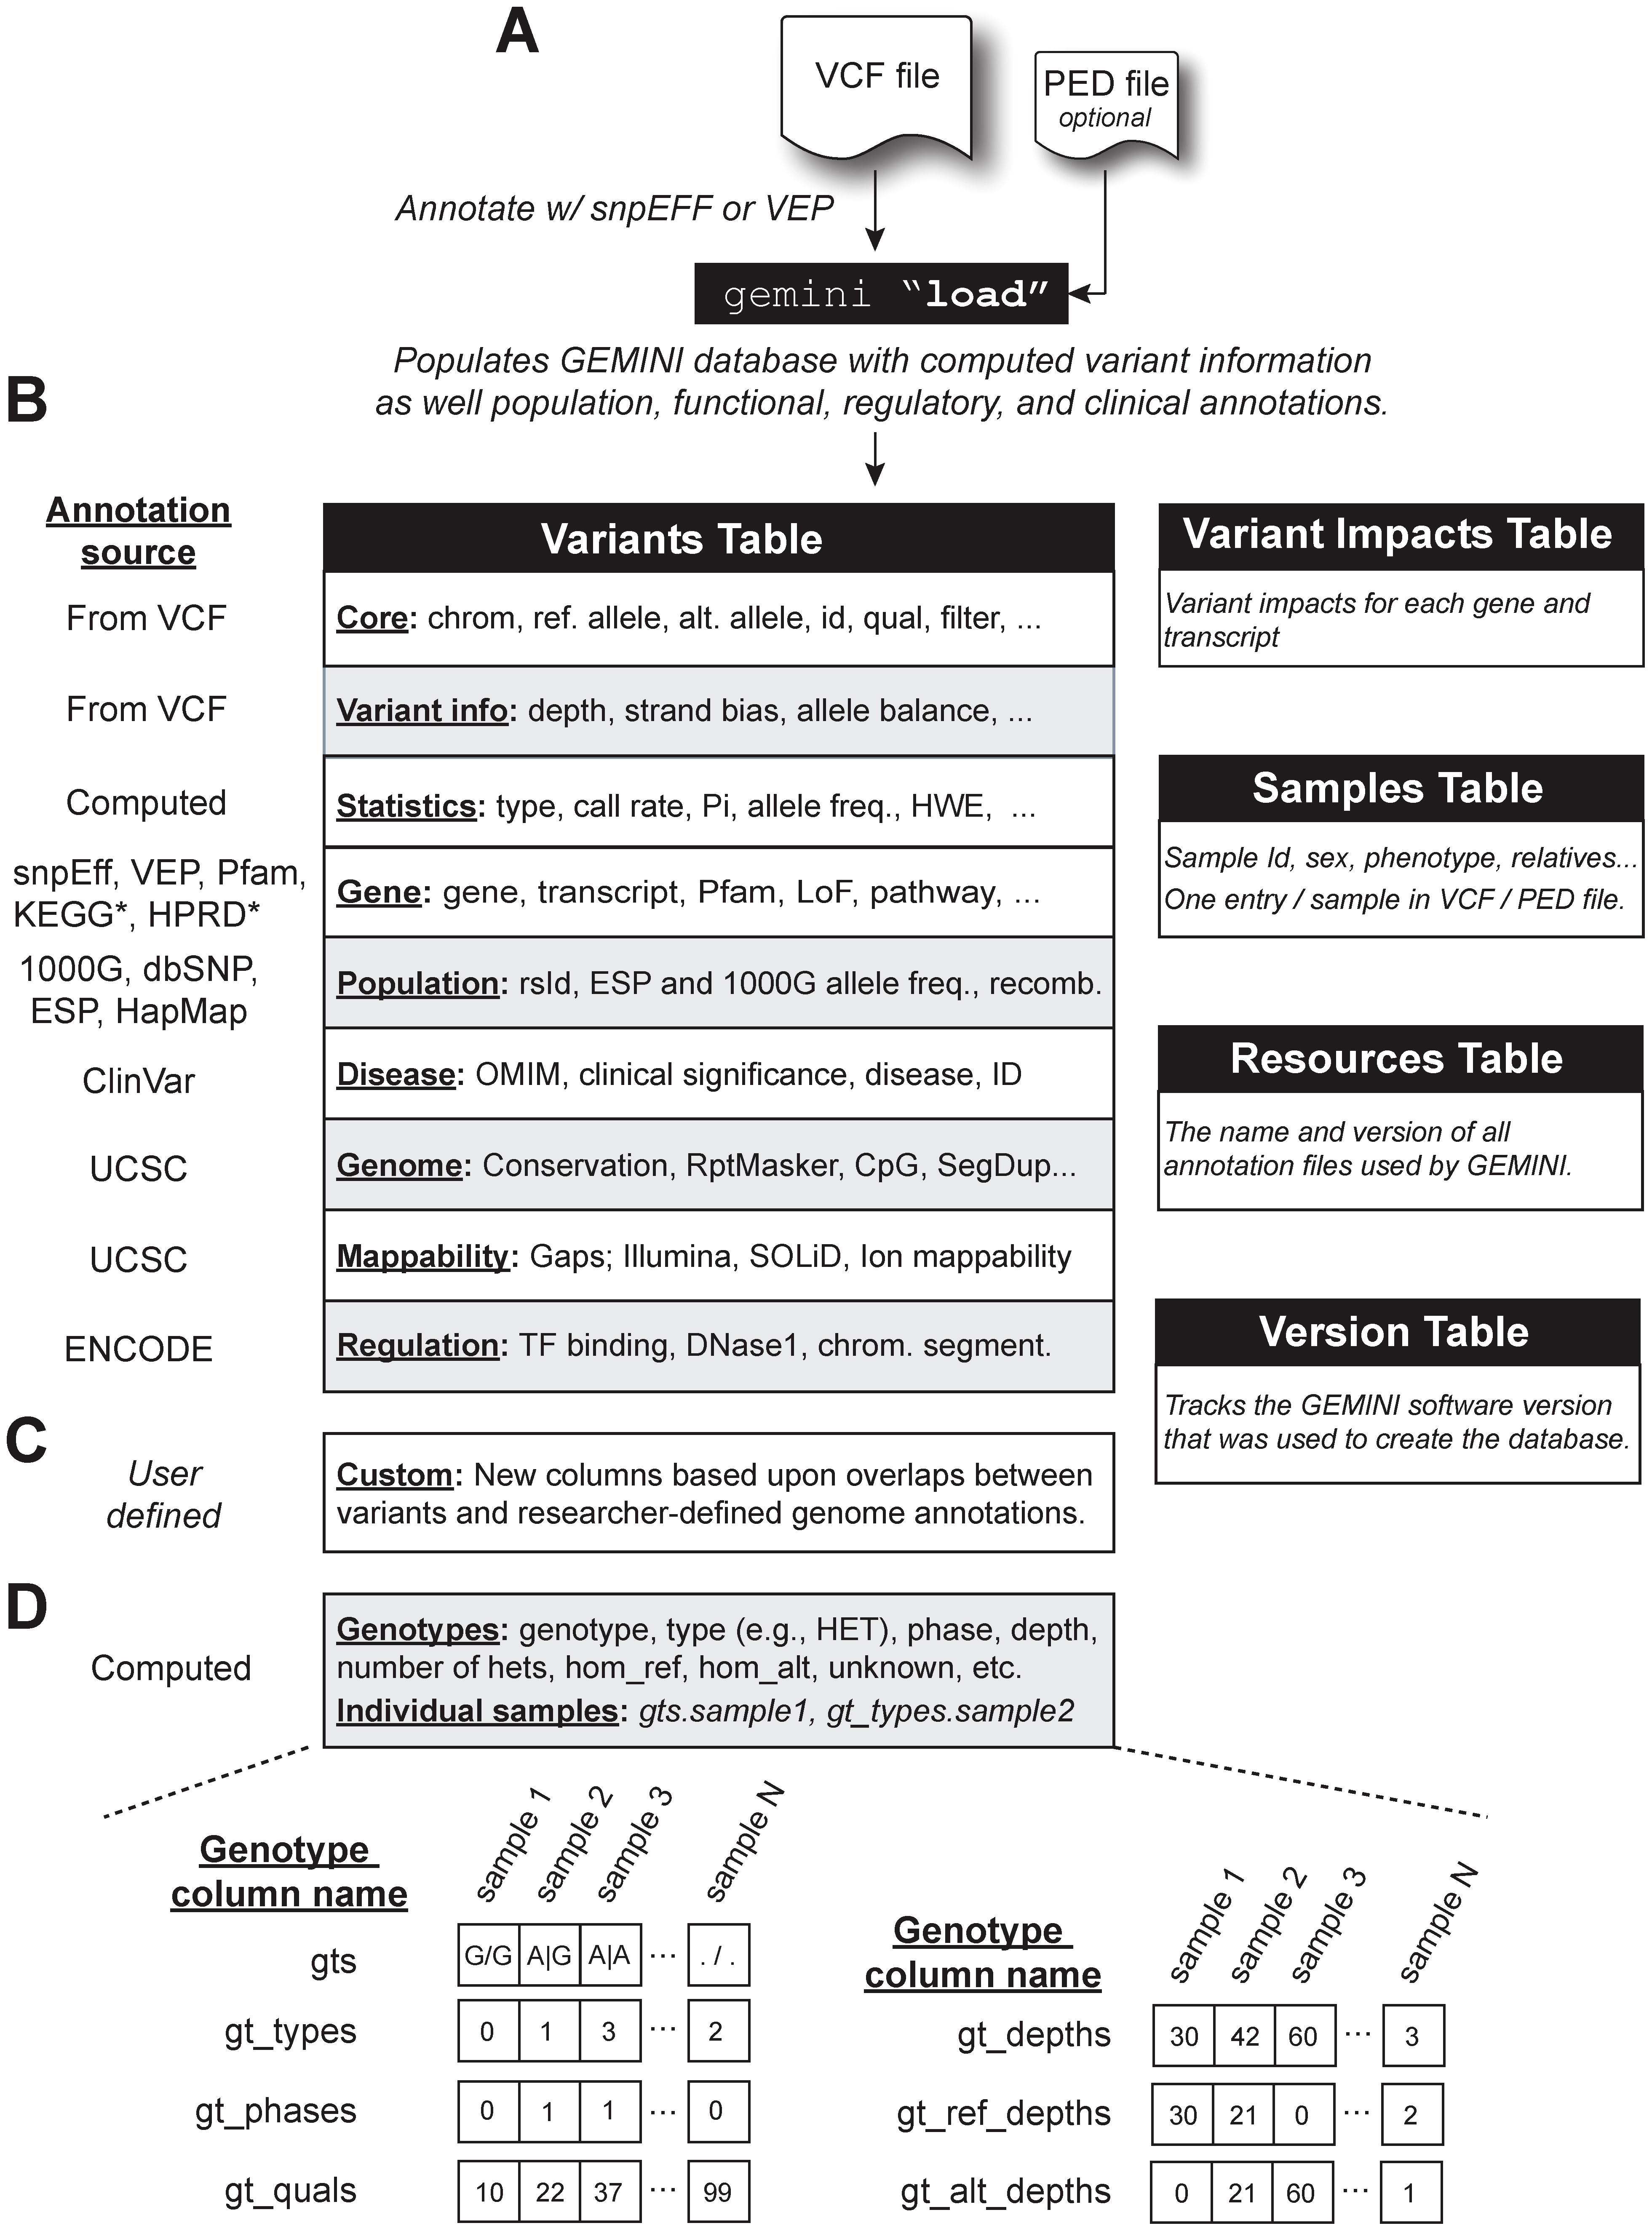
\includegraphics[scale=0.8]{gemini_schema}
\caption{Een overzicht van GEMINI's schema}
\label{gemini_schema_pic}
\end{figure}

\section{Inladen}
%TODO ref nr IPython dink
Het inladen van de data uit VCF-bestanden is een computationeel intensieve operatie, enerzijds omwille van de enorme grootte van deze bestanden, en anderzijds omdat in deze fase ook alle variants geannoteerd moeten worden. Om het proces te versnellen, biedt GEMINI de mogelijkheid het werk te paralleliseren door het VCF-bestand de comprimeren, op het bestaande bestand een index te defini\"eren en zo het werk te verdelen. Dit kan simpelweg over meerdere processoren binnen 1 computer zijn, maar via de IPython-interface ook over volledige clusters van computers.\\



\chapter{Oplossing}
\label{oplossing}

Dit hoofdstuk belicht aan de hand van een case-study de praktische realisatie van een schaalbare tool voor software-analyse. De case-study in kwestie is een implementatie van GEMINI die werkt met een Cassandra i.p.v. SQLite databank. Achtereenvolgens komen een motivatie voor de keuze voor Cassandra, de nodige aanpassingen aan het dataschema van GEMINI, en de nodige aanpassingen aan de implementatie van de querying-functionaliteit van GEMINI aan bod.

\section{Keuze database}

\subsection{Vereisten}

Zoals beschreven in [\ref{gemini_beschrijving}] bewaart GEMINI de data over genetische varianten en proefpersonen in enkele zeer grote tabellen. Een eerste vereiste voor een database is dus om deze tabulaire data goed te kunnen voorstellen en beheren. Omdat de nadruk van dit onderzoek specifiek ligt op het schaalbaar maken van de applicatie, gebeurt dit bij voorkeur d.m.v. automatische verspreiding over verschillende nodes in een cluster.\\
Omdat GEMINI meerdere processoren of zels computers kan gebruiken bij het inladen van de gegevens uit VCF-bestanden, is goede concurrency controle en hoge schrijf-throughput eveneens belangrijk. Na het inladen van de VCF bestanden voert GEMINI enkel nog lees-queries uit, dus zijn de belangrijkste verdere vereisten voor een database hoge lees-throughput, goede query-mogelijkheden en indexeringsmechanismes.
\\Ten laatste is een Python-API ook nuttig, gezien GEMINI in Python ge\"implementeerd is.

\subsection{Keuze}

De uiteindelijke keuze voor een databank viel op Apache Cassandra. Van de systemen besproken in [\ref{nosql_survey}] heeft Cassandra veruit de meest interessante architectuur qua schaalbaarheid en bovendien leent het columnaire model zich goed tot het modelleren van de tabellen in de oorspronkelijke versie van GEMINI. Vergeleken met het andere columnaire systeem, HBase, heeft Cassandra uitgebreidere query-mogelijkheden. Vergeleken met MongoDB, dat sterker staat op het gebied van querying en indexing heeft Cassandra het voordeel dat het flexibeler is voor concurrent schrijven naar de databank. Bovendien blijkt uit eerdere experimenten met MongoDB binnen het lab dat MongoDB niet space-effici\"ent BSON-documenten kan uitbreiden. In het geval van een incrementele versie van GEMINI, waar na verloop van tijd genoominformatie van extra proefpersonen ingeladen moet worden, leidt dit tot fragmentatie. Cassandra daarentegen kan eenvoudig het schema van tabellen aanpassen en naar behoefte extra kolommen en rijen toevoegen.\\
Zoals later uitgebreid aan bod komt, heeft Cassandra ook nadelen. Vooral de eerder beperkte query-capaciteiten bemoeilijken het implementeren van de uitgebreide ad-hoc queryfunctionaliteiten van GEMINI.

\section{Dataschema GEMINI in Cassandra}
\label{cassandra_datamodel}

Het datamodel van Apache Cassandra vertoont enkele sterke verschillen met het relationele datamodel. Dit vereist enkele grondige aanpassingen aan het database schema van GEMINI. In deze sectie komen de belangrijkste eigenschappen van Cassandra aan bod, hun gevolgen voor de belangrijkste database-functionaliteiten, en de uitgevoerde aanpassingen aan het onderliggende schema van GEMINI ten op zichte van de SQLite implementatie.

\subsection{Datamodel Cassandra}

Zoals eerder vermeld bewaart Cassandra de cellen in een tabel als een 2 dimensionele map van enerzijds een per rij gedefinieerde primary key, en de naam van een kolom. De inhoud van cellen die niet in de primary key van een rij liggen, heeft voor Cassandra geen enkele betekenis.\\
Die primary key bestaat uit 2 delen: het eerste is de partition key, deze bestaat uit minstens 1 kolom en de waarde hiervan die via het consistent-hashing mechanisme bepaalt op welke partitie in het cluster de rij terechtkomt. Het tweede, optionele, deel is de clustering key, en bepaalt in welke volgorde rijen met dezelfde partition key op 1 node bewaard worden. Dit is standaard in oplopende volgorde.\\\\

%TODO: ALLOW FILTERING
Omdat het inspecteren van cellen indruist tegen de principes van Cassandra, zijn de query-mogelijkheden eerder beperkt: zonder het defini\"eren van indices is het in \texttt{WHERE}-clausules enkel mogelijk beperkingen op te leggen aan kolommen in de primary key, en dan nog zo dat de bedoelde rijen binnen 1 partitie liggen, en opeenvolgend opgeslagen zijn. Daarom moet er een gelijkheidsbeperking opgelegd worden aan de volledige partition key, en mogen er zowel gelijk- als ongelijkheidsbeperkingen opgelegd worden aan de kolommen in de clustering key, maar enkel op voorwaarde dat de voorgaande kolom in de clustering key ook met een gelijkheidsbeperking gespecifieerd is. Op deze manier kan Cassandra queries zeer snel uitvoeren door ze a.d.h.v. de hash van de partition key naar een juiste node te routeren, en vervolgens via de overige opgegeven kolommen de locatie van de juiste rijen te berekenen (die omwille van de clustering allemaal opelkaar volgend opgeslagen zijn). Dit gebeurt zonder de waarden van individuele cellen te bekijken, maar dus enkel door het berekenen van een simpele hashfunctie. Range-queries zijn dus enkel mogelijk op kolommen in de clustering key en het is niet mogelijk \texttt{!=}-beperkingen te gebruiken in \texttt{WHERE}-clausules. Bovendien laat Cassandra enkel toe beperkingen met elkaar te combineren via conjuncties, dus niet via \texttt{OR}- of \texttt{NOT}-operatoren. Een uitzondering op dit laatste is de \texttt{IN}-operator: op deze manier kan de gebruiker meegeven in welke set van waarden een bepaalde kolom moet liggen, maar dit is ook enkel mogelijk op de laatste kolom in de partition key of de laatste kolom in de clustering key (maar weer op voorwaarde dat de voorgaande kolommen reeds beperkt zijn).\\
Cassandra laat toe om indices op kolommen te defini\"eren, maar deze zijn niet bijzonder nuttig. Ze laten enkel gelijkheidsbeperkingen toe (dus geen range-queries) en bovendien raadt Datastax het gebruik van indices op kolommen met zowel een zeer lage als een zeer hoge kardinaliteit af, dit omdat in het eerste geval de index tabel zal bestaan uit zeer weinig zeer lange rijen voor elk van de ge\"indexeerde waarden en in het tweede geval Cassandra bij een query op de ge\"indexeerde kolom door zeer veel verscheidene waarden zal moeten zoeken om een klein aantal resultaten te vinden \cite{when_to_use_index}.

\subsection{Databaseschema GEMINI}
Zoals blijkt uit bovenstaande beschrijving van het datamodel van Cassandra, leent het systeem zich niet goed tot ad-hoc querying: het is niet mogelijk op een performante manier zomaar aan willekeurige kolommen in een tabel voorwaarden op te leggen en deze voorwaarden met elkaar te combineren. Dit betekent dat bij het ontwerpen van het database schema al rekening gehouden moet worden met de queries die achteraf op de data mogelijk moeten zijn. Omdat het soort queries dat een tabel ondersteunt sterk samenhangt met de keuze van de primary key van de tabel en GEMINI meerdere, uiteenlopende soorten queries op elke tabel vereist, zal dit onvermijdelijk leiden tot duplicatie van data.

\paragraph{\texttt{variants}-tabel vs. genotype-informatie}

Het belangrijkste vraagstuk is hoe de genotype-kolommen uit het oorspronkelijke relationele model in Cassandra op te slaan. Hier zijn enkele opties voor:

\begin{itemize}

\item \textbf{Collection columns} Cassandra biedt zogenaamde collection types, zoals sets, lists of maps. Dit is vergelijkbaar met de bestaande implementatie in SQLite (buiten dat ze in Cassandra niet als binary blobs bewaard worden). Het nadeel is echter dat deze collections niet meer dan 65536 ($2^{16}$) entries kunnen bevatten, wat het hele nut van de migratie naar Cassandra zou ondermijnen.

\item \textbf{Super-\texttt{variants}-tabel} Een andere mogelijkheid is de \texttt{variants}-tabel uit te breiden met een kolom voor elke genotype-eigenschap van elke sample. Deze aanpak heeft als voornaamste voordeel dat de kolommen met genotype-eigenschappen van specifieke samples zonder omwegen uit de \texttt{variants}-tabel gehaald kunnen worden. Dit is vooral van belang voor de in (\ref{gemini_beschrijving}) beschreven sample-filters. Bovendien kan Cassandra tot 2 miljard cellen opslaan op 1 partitie, dus vormt het grote aantal kolommen dat dit model met zich meebrengt, geen probleem.\\
Het nadeel is echter dat het onmogelijk is ad-hoc queries te defini\"eren op genotypes van willekeurige eigenschappen zonder het gebruik van secundaire indices. Elke query die in een \texttt{WHERE}-clausule andere kolommen of samples betrekt, vereist om de hierboven beschreven redenen een andere keuze van de primary key om effici\"ent de juiste rijen te kunnen opzoeken.

\begin{table}[!htbp]
\begin{tabular}{@{}|l|l|l|l|l|l|l|l|l|l|@{}}
\toprule
\color{green} variant\_id & ref & alt & \ldots & gt\_type\_alex & gt\_type\_john & \ldots & gt\_depth\_alex & gt\_depth\_john & \ldots \\ \bottomrule
\end{tabular}
\end{table}

\item \textbf{\texttt{genotype}-tabellen} Een derde optie is een \texttt{variants}-tabel zonder genotype-informatie, gecombineerd met een tabel voor elke eigenschap van de genotypes van de samples, met een rij voor elke \texttt{(variant, sample)}. Bijvoorbeeld:\\

\begin{itemize}

\item Een \texttt{variants\_by\_samples\_gt}-tabel met als primary key \texttt{((sample\_name, gt\_type), (variant\_id))}. De primary key is zo gekozen dat alle variants waarvoor een sample eenzelfde genotype heeft, bij elkaar op 1 node liggen, zodat deze gemakkelijk opgevraagd kunnen worden. Hetzelfde was mogelijk geweest met enkel \texttt{sample\_name} als partition key, maar met de bovenstaande, granulairdere partition key zijn de variants beter over het cluster verspreid. Bovendien houdt het vanuit een semantisch oogpunt geen steek range queries uit te voeren op de \texttt{gt\_type}-kolom, dus moet deze niet per se in de clustering key staan. De \texttt{variant\_id}-kolom ten slotte maakt enkel deel uit van de primary key om deze uniek te maken voor elk tupel \texttt{(variant, sample, genotype)}.\\

\begin{table}[!htbp]
\begin{tabular}{@{}|l|l|l|@{}}
\toprule
\color{green} sample\_name & \color{green} genotype & \color{red} variant\_id \\ \bottomrule
\end{tabular}\\
\end{table}

\item Een \texttt{variants\_by\_samples\_gt\_depth}-tabel met als primary key \texttt{((sample\_name), (gt\_depth, variant\_id))}. Omdat range queries op de \texttt{gt\_depth}-kolom wel een vereiste zijn, moeten alle variants voor eenzelfde sample volgens gt\_depth geclusterd, en dus gerangschikt staan. Vandaar dat de \texttt{gt\_depth}-kolom in dit geval in de clustering key, en niet in de partition key staat. Voor de rest is de keuze van de primary key volledig analoog met die in de \texttt{variants\_by\_samples\_gt}-tabel.

\begin{table}[!htbp]
\begin{tabular}{@{}|l|l|l|@{}}
\toprule
\color{green} sample\_name & \color{red} gt\_depth & \color{red} variant\_id \\ \bottomrule
\end{tabular}
\end{table}

\item Vergelijkbare tabellen voor de overige genotype-eigenschappen.

\end{itemize}

Het grote voordeel van deze aanpak is dat het, dankzij de keuze van de primary key, zeer eenvoudig is variants op te vragen waarvoor het genotype van \'e\'en sample aan specifieke gelijkheids- of ongelijkheidsvoorwaarden voldoet. Het nadeel van dit schema is drieledig: ten eerste scheidt het de informatie over de genotypes van samples van de andere informatie over de variants. Dit betekent dat, om deze samen weer te geven, een \texttt{JOIN} van de \texttt{variants}-tabel met een \texttt{genotype}-tabel nodig is, en Cassandra biedt zoals geweten geen \texttt{JOIN}. Ten tweede is het onmogelijk om met een sample-filter voor meerdere samples de genotypes tegelijkertijd op te vragen, en ten laatste is het onmogelijk in een query voorwaarden op te leggen aan de genotypes van meerdere samples.


\end{itemize}

De uiteindelijke keuze is gevallen op een combinatie van de tweede en derde optie. Dit om de volledige oorspronkelijke functionaliteit van GEMINI te kunnen bieden: enerzijds het opvragen van de genotype-informatie van willekeurige samples door middel van de sample-filters, en anderzijds het query'en van de \texttt{variants}-tabel met, dankzij gt-filters en -wildcards, beperkingen op de genotypes van specifiek gekozen samples. Zoals hierboven beschreven is dit laatste niet voor de hand liggend, en zal door het ontbreken van \texttt{JOIN}s en de layout van de \texttt{genotype}-tabellen het combineren van beperkingen op de genotypes van meerdere samples nog extra aanpassingen vergen. Hier komt sectie \ref{??} uitgebreid op terug.
%TODO 

\paragraph{\texttt{variants-, samples-}tabel vs. arbitraire queries}

Een tweede belangrijke vraagstuk is hoe de \texttt{variants-} en \texttt{samples-}tabellen zo te ontwerpen dat ze ook op andere, arbitraire kolommen effici\"ent doorzoekbaar zijn.\\
Om queries op kolommen te ondersteunen die logisch gezien enkel met gelijkheden beperkt zullen worden, zoals \texttt{chrom} of respectievelijk \texttt{sex}, zou het in theorie volstaan op deze kolommen een secundaire index te defini\"eren. Dit is eenvoudig bij de creatie van de tabel, veroorzaakt geen duplicatie van data en is zeer rechttoe-rechtaan bij het query'en, maar heeft zoals hierboven vermeld onvoorspelbare performantie afhankelijk van de kardinaliteit van de kolommen. Bovendien werkt dit mechanisme niet voor kolommen die vaker met ongelijkheidsbeperkingen gequeried zullen worden, zoals \texttt{depth}, \texttt{start}, of in het geval van de \texttt{samples}-tabel (hypothetisch, deze tabellen zitten niet standaard in GEMINI) leeftijd of generatie.\\

Een aanpak die in beide gevallen op een voorspelbare en betrouwbare manier werkt, is om net als voor de genotype-informatie extra tabellen te defini\"eren, met een specifiek gekozen primary key die de gewenste query mogelijk maakt. Deze oplossing zorgt natuurlijk voor veel gedupliceerde data, maar heeft als voordeel dat ze \'e\'en coherente en performante aanpak van het probleem mogelijk maakt. Bij het opstellen van deze tabellen moet goed overwogen worden welke vaakgebruikte queries een eigen tabel vereisen en verdienen. Minder frequente, uitgebreidere queries, kunnen mits een goede keuze van de basistabellen immers gesplitst worden in subqueries op deze basistabellen. Hetzelfde mechanisme dat voor de gt-filters en -wildcards uitgebreide queries zal uitvoeren is ook hier van toepassing. Dit zal natuurlijk minder effici\"ent zijn dan een aangepaste tabel voor de uitgebreide, originele query, maar laat toe de data-duplicatie enigszins binnen de perken te houden. Voorbeelden van zulke basistabellen zijn:

\begin{itemize}
\item Een \texttt{variants\_by\_chrom\_start}-tabel, die het eenvoudig maakt alle varianten op te zoeken die op een bepaald chromosoom binnen een range van startposities liggen. De primary key is in dit geval: \texttt{((chrom), (start, variant\_id))}. 

\begin{table}[!htbp]
\begin{tabular}{@{}|l|l|l|@{}}
\toprule
\color{green} chrom & \color{red} start & \color{red} variant\_id \\ \bottomrule
\end{tabular}
\end{table}

\item Een \texttt{variants\_by\_gene}-tabel, die het eenvoudig maakt alle varianten binnen \'e\'en gen op te zoeken. De primary key is in dit geval: \texttt{((gene), (variant\_id))}.

\begin{table}[!htbp]
\begin{tabular}{@{}|l|l|@{}}
\toprule
\color{green} gene & \color{red} variant\_id \\ \bottomrule
\end{tabular}
\end{table}

\item Een \texttt{samples\_by\_sex}-tabel, die het eenvoudig maakt alle samples van een bepaald geslacht op te vragen. De primary key is in dit geval: \texttt{((sex), (sample\_name))}.

\begin{table}[!htbp]
\begin{tabular}{@{}|l|l|@{}}
\toprule
\color{green} sex & \color{red} sample\_name \\ \bottomrule
\end{tabular}
\end{table}
\end{itemize}

Ten slotte is het ook nog interessant een feature aan de GEMINI command line interface toe te voegen waarmee de gebruiker zelf nieuwe basistabellen kan defini\"eren wanneer hij dit nodig acht.

\section{Implementatie GEMINI vs. Cassandra}

\subsection{\texttt{gemini load}}

Het inladen van genoomdata in GEMINI gebeurt in twee stappen. De reden voor deze opsplitsing is dat een klein deel van het inladen en initialiseren van de databank niet parallel op meerdere processoren kan verlopen. \\In de eerste en kleinste van de twee, initialiseert GEMINI de databank, maakt de nodige tabellen aan en laadt de samples-informatie in. GEMINI haalt de namen van de samples uit de VCF-file, en vult deze aan met informatie uit de ped-file. Indien er geen ped-file voorhanden is, initialiseert GEMINI de \texttt{samples}-tabel met default-waarden voor de kolommen zoals \texttt{sex} en \texttt{phenotype}. Meteen worden ook de extra, aan de \texttt{samples}-tabel verbonden tabellen zoals \texttt{samples\_by\_sex} en \texttt{samples\_by\_phenotype} aangemaakt en gevuld. Ook de \texttt{resources-, gene\_detailed-, gene\_summary-} en \texttt{version-}tabellen worden in deze fase gevuld. Dit omdat de pedigree-files en de bestanden met data over de genen niet effici\"ent opgesplitst kunnen worden. Bovendien is de duur van het inladen van de \texttt{samples}-tabel zelfs bij 10000'en samples verwaarloosbaar tegenover het inladen en annoteren van de \texttt{variants}-tabel.\\

In de tweede fase gebeurt het leeuwendeel van het werk: het inladen van de variants-informatie uit de (verplicht meegegeven) VCF-file. Dankzij de bgzip \cite{bgzip} en grabix \cite{grabix} tools kan GEMINI effici\"ent VCF-bestanden in blokken opsplitsen, comprimeren, hierop een index defini\"eren en vervolgens daarmee verderwerken. Zo kan GEMINI eenvoudig het inladen van de variants, die elk \'e\'en lijn in de VCF-file in beslag nemen, gemakkelijk over meerdere cores verdelen. Het is uiteraard ook in deze fase dat GEMINI de aan de \texttt{variants}-tabel verwante tabellen zoals \texttt{variants\_by\_samples\_gt\_type}, \texttt{variants\_by\_samples\_gt\_depth} en \texttt{variants\_by\_chrom\_start} opvult. Alle cores of nodes in het cluster, voeren rechtstreeks rijen in in \'e\'en en dezelfde tabel in de Cassandra-databank. Omdat Cassandra atomiciteit binnen rijen garandeert en alle workers strikt disjuncte sets van variants invoeren in het systeem, is er geen enkel risico op conflicten.\\\\
De grote winst ten opzichte van de SQLite-implementatie van GEMINI is dat in het parallelle gedeelte, alle workers naar dezelfde databank kunnen schrijven. In de SQLite-versie van GEMINI schrijven alle workers naar een aparte SQLite-database, die vervolgens in een kostelijke operatie nog allemaal samengevoegd moeten worden tot \'e\'en grote SQLite-databank. Deze stap (het \texttt{gemini merge}-commando) kan de Cassandra-implementatie volledig overslaan. Een ander opzicht waarin de Cassandra-implementatie effici\"enter is dan de SQLite-versie, is dat in SQLite voor elke variant de genotype-kolommen nog tot binary blobs gecomprimeerd worden. In Cassandra is dit, dankzij de keuze van het databaseschema, niet nodig.
 
\subsection{\texttt{gemini query}}

Het uitvoeren van de gewoonlijke GEMINI-queries tegen een Cassandra-databank vergt enkele ingrijpende aanpassingen ten opzichte van de SQLite-versie van Cassandra. Het doel is natuurlijk deze aanpassingen zoveel mogelijk te verbergen voor de gebruiker, wat ook in grote mate gelukt is. In deze sectie komt achtereenvolgens aan bod hoe ingewikkelde queries gesplitst worden in eenvoudige subqueries, hoe de resultaten hiervan vervolgens gecombineerd worden en wat dit betekent voor de meest geavanceerde feature van GEMINI, namelijk de genotype-filter wildcards.

\paragraph{Reductie tot subqueries}

Zoals beschreven in \ref{cassandra_datamodel}, kan Cassandra enkel effici\"ent queries uitvoeren die beperkingen opleggen aan de kolommen in de primary key van een tabel, en dit ook slechts onder bepaalde voorwaarden. Bovendien is de enige logische operator die Cassandra ondersteunt om beperkingen te combineren, de conjunctie.\\
Om arbitraire queries en \texttt{WHERE}-clausules te ondersteunen, kan GEMINI niet zoals in de SQLite-versie de \texttt{WHERE}-clausule zomaar onveranderd aan Cassandra doorgeven. Om dit te illustreren, zal ik de onderstaande query als voorbeeld hanteren:\\\\
\texttt{SELECT chrom, start, subtype FROM variants WHERE chrom = 'chromX' AND start > 5600 AND gene = 'gene\_A'}.\\\\
Deze query valt uiteen in 2 subqueries: een eerste om uit de \texttt{variants\_by\_chrom\_start}-tabel alle variants op te vragen die voldoen aan de voorwaarde \texttt{chrom = 'chromX' AND start > 5600} en een tweede om uit de \texttt{variants\_by\_gene}-tabel alle variants die voldoen aan \texttt{gene = 'gene\_A'} op te vragen.\\

Om beslissingen zoals in het voorbeeld dynamisch te kunnen maken, is het nodig de \texttt{WHERE}-clausule te inspecteren en hieruit de benodigde hulptabellen voor de subqueries te identificeren. Om dit proces te vereenvoudigen, heb ik ervoor gekozen de query syntax licht aan te passen: beperkingen die binnen 1 hulptabel liggen, kunnen nog steeds met elkaar gecombineerd worden met het \texttt{AND}-keyword, maar beperkingen die niet binnen eenzelfde hulptabel liggen, moeten met de \texttt{\&\&, ||} of \texttt{NOT}-operatoren van elkaar gescheiden worden. Zo kan GEMINI bij het parsen van de \texttt{WHERE}-clausule deze onmiddellijk opsplitsen in subqueries en voor elk van deze subqueries de nodige hulptabel bepalen. Zo wordt de voorbeeldquery:\\\\
\texttt{SELECT chrom, start, subtype FROM variants WHERE chrom = 'chromX' AND start > 5600 \&\& gene = 'gene\_A'}.\\

Dit vereist van de gebruiker uiteraard dat hij op de hoogte is van welke hulptabellen er bestaan. Gebruikers moeten sowieso weten op welke kolommen ze queries kunnen defini\"eren, en bijgevolg ook welke hulptabellen er bestaan. Bovendien bestaat het doelpubliek van GEMINI uit onderzoekers die het programma intensief gebruiken en dus voldoende gelegenheden hebben om dergelijke aanpassingen snel onder de knie te krijgen.\\
%TODO
Een andere optie is de syntax onveranderd te laten en uit de in de \texttt{WHERE}-clausule vermelde kolommen benodigde hulptabellen af te leiden. Deze aanpak heeft als voordeel dat de interface naar de gebruiker niet verandert, maar gezien nog steeds enkel queries mogelijk zijn op kolommen uit de hoofdtabel waarvoor hulptabellen bestaan, is achterwaartse compatibiliteit hiermee nog niet verzekerd. Daarbovenop levert deze aanpak ook nieuwe problemen op, zoals: wat met kolommen die in meerdere hulptabellen voorkomen, welke combinatie van tabellen wordt er dan best geselecteerd? Dergelijke vraagstukken neigen naar query-optimization en vallen buiten het ... Daarom verkoos ik de macht bij de gebruiker te leggen en te vertrouwen op diens oordeelkundigheid.\\\\
De gebruiker dient er ook rekening mee te houden dat Cassandra range-queries enkel onder strikte voorwaarden ondersteunt, namelijk (zoals eerder uitgelegd) enkel op clustering columns en enkel wanneer de voorgaande kolommen in de clustering key met gelijkheden beperkt zijn. Dit impliceert dat er slechts een range query op 1 kolom in een tabel mogelijk is. Daarnaast biedt Cassandra ook geen \texttt{!=}-operator. Dit euvel valt te verhelpen door een \texttt{!=}-clausule om te zetten naar een gelijkheidsbeperking en deze vervolgens te negeren (zie volgende paragraaf voor evaluatie van negaties). Een clausule als \texttt{phenotype != 2} wordt dan \texttt{NOT (phenotype = 2)}. Dit vereist dat de \texttt{!=}-clausule een aparte subquery vormt.\\

Het uiteindelijke algoritme om de juiste hulptabel te identificeren op basis van de kolommen en gebruikte operatoren in een subquery, gebruikt de metadata van het Cassandra-cluster om alle hulptabellen voor een gegeven hoofdtabel op te vragen, en vervolgens aan de hand van de kolommen in de primary keys van de kandidaat-hulptabellen de geschikte eruit te kiezen.
%TODO code?

\paragraph{Combineren subqueries}

\textbf{conceptueel}
De subqueries zullen elk een verzameling rijen als resultaat opleveren. Het is dan zaak deze verzamelingen met set-operaties te combineren tot de finale verzameling rijen die aan de query voldoen. De nodige set-operatie hangt af van de oorspronkelijke query. Zo zal het eindresultaat van een conjunctie van subqueries de doorsnede van de resultaatverzamelingen van de subqueries zijn. In het geval van een disjunctie is dit de unie van de resultaatverzamelingen, en in het geval van een negatie van een subquery is dit het verschil tussen de oorspronkelijke verzameling (voor de query) en de resultaatverzameling van de query. Om bijvoorbeeld alle varianten te vinden die niet op een bepaald gen x liggen, moet het verschil bepaald worden tussen de verzameling van alle varianten en de verzameling van alle varianten die op gen x liggen. Onderstaande tabel vat dit samen voor 2 subqueries $p$ en $r$, hun respectievelijke resultaatverzamelingen $res(p)$ en $res(r)$ en een initi\"ele verzameling rijen $I$.

\begin{table}[h]
\centering
\begin{tabular}{|l|l|}
\hline
\textbf{Query} & \textbf{Resultaat}    \\ \hline
$p$ \texttt{AND} $r$ & $res(p) \cap res(r)$   \\ \hline
$p$ \texttt{OR} $r$ & $res(p) \cup res(r)$    \\ \hline
\texttt{NOT} $p$  & $I \setminus res(p)$ \\ \hline
\end{tabular}
\end{table}

\textbf{praktisch}

Uit performantie-overwegingen is het een logische keuze de resultaten van subqueries op de hulptabellen te bewaren in een set datatype. Zo kunnen de benodigde set-operaties gebruik maken van de in Python ingebouwde set-operaties en zo veel effici\"enter verlopen dan wanneer de resultaten in bijvoorbeeld lists bewaard worden. Het enige nadeel van sets t.o.v. lists is dat de implementatie geen garanties biedt over in welke volgorde rijen in het eindresultaat zullen voorkomen. Dit weegt niet op tegen de tijdswinst, en bovendien biedt Cassandra zelf in het algemeen geen enkele garantie over in welke volgorde het rijen opslaat.\\\\
Bij het praktisch evalueren van \texttt{query\_expression}s komt uiteindelijk meer kijken dan enkel set-operaties. De belangrijkste reden hiervoor is dat, zoals in ?? %TODO
reeds beschreven, om een \texttt{NOT\_expression} te kunnen evalueren, alle kandidaat-rijen gekend moet zijn, en dus meegegeven aan de \texttt{evaluate}-functie. Deze extra informatie kan ook bij het evalueren van andere types van \texttt{query\_expression} goed van pas komen.
 
\begin{itemize}
\item Het evalueren van \texttt{Basic\_expression}s gebeurt niet zo rechtoe rechtaan als de naam doet vermoeden. De \texttt{evaluate}-functie bouwt een CQL-query op, op basis van een gegeven \texttt{WHERE}-clausule, de relevante tabel en de gevraagde kolom uit die tabel. Wanneer er een zinvolle verzameling kandidaatrijen (de \texttt{starting\_set} in onderstaand codefragment) meegegeven is, wordt deze als \texttt{IN}-clausule aan de \texttt{WHERE}-clausule toegevoegd. Zo zoekt Cassandra enkel in rijen die effectief in aanmerking komen om aan de globale query te voldoen. Een voorwaarde om deze optimalisatie te kunnen toepassen, is dat de \texttt{WHERE}-clausule geen ongelijkheidsbeperkingen mag bevatten (vandaar de \texttt{can\_prune}-functie).

\lstinputlisting[language=Python,firstline=31,lastline=31]{../gemini/gemini/query_expressions.py}
%TODO juist formatten, binnenste if, else verstoppen
\lstinputlisting[language=Python,firstline=36,lastline=53]{../gemini/gemini/query_expressions.py}

\item Om een \texttt{AND\_expression} te evalueren is het strikt genomen nodig beide leden van de uitdrukking te evalueren en vervolgens de doorsnede te nemen van de resultaten. Als \'e\'en van de twee leden van de uitdrukking echter in staat is om dankzij een CQL \texttt{IN}-clausule enkel naar rijen te zoeken die effectief in aanmerking komen om aan de globale query te voldoen, is het mogelijk om deze operatie aan Cassandra over te laten. Als het rechterlid kan \textit{prunen}, dan kan GEMINI de resultaatverzameling van het linkerlid als \texttt{starting\_set} meegeven bij de evaluatie van het rechterlid, en omgekeerd. Wanneer geen van beide kunnen \textit{prunen}, moet GEMINI uiteraard nog steeds zelf de doorsnede berekenen.

\lstinputlisting[language=Python,firstline=64,lastline=64]{../gemini/gemini/query_expressions.py}
\lstinputlisting[language=Python,firstline=69,lastline=77]{../gemini/gemini/query_expressions.py}

\item In het geval van een \texttt{OR\_expression} is er geen andere mogelijkheid dan eenvoudigweg het linker- en rechterlid te evalueren, beide met als \texttt{starting\_set} de \texttt{starting\_set} van de \texttt{OR\_expression} zelf, en vervolgens de unie van de resultaten te berekenen.

\item Ook in het geval van een \texttt{NOT\_expression} is er geen andere optie dan de \texttt{body}-uitdrukking te evalueren en vervolgens het complement van de \texttt{starting\_set} en het resultaat te bepalen. Als de gegeven \texttt{starting\_set} gelijk is aan \texttt{"*"}, d.w.z. alle rijen in de oorspronkelijke tabel, zit er ook niets anders op dan deze nog eerst allemaal op te vragen.

\lstinputlisting[language=Python,firstline=112,lastline=112]{../gemini/gemini/query_expressions.py}
\lstinputlisting[language=Python,firstline=116,lastline=123]{../gemini/gemini/query_expressions.py}

\end{itemize}

Een optimalisatie die voor alle \texttt{query\_expressions} geldt is dat in het geval van een lege \texttt{starting\_set}, GEMINI de hele evaluatie kan overslaan. Dit bespaart een overtollige round-trip naar de Cassandra-databank. Voor alle soorten \texttt{query\_expressions} behalve \texttt{Basic\_expression} geldt ook dat ze kunnen \textit{prunen}, ongeacht de aard van hun subqueries. In het geval dat hun subqueries een \texttt{Basic\_expression} bevatten die niet kan \textit{prunen}, zal de subquery in kwestie dit zelf afhandelen bij de evaluatie.

\paragraph{Genotype-filter wildcards}

\textbf{conceptueel}
Ter herinnering, de structuur van een genotype-filter wildcard:\\\\
\texttt{(genotype\_column).(sample\_wildcard).(gt\_wildcard\_rule).(rule\_enforcement)}\\\\
Het uitvoeren en evalueren van deze wildcards is conceptueel niet erg ingewikkeld: het volstaat de \texttt{sample\_wildcard} te evalueren en vervolgens voor elk van de resulterende samples een subquery op te stellen op de voor \texttt{genotype\_column} relevante hulptabel van de \texttt{variants}-tabel. Hoe deze subqueries met elkaar gecombineerd moeten worden, hangt af van de gegeven \texttt{rule\_enforcement}:

\begin{itemize}
\item Een \texttt{all}-wildcard leidt tot de conjunctie van alle subqueries.
\item Een \texttt{any}-wildcard leidt tot de disjunctie van alle subqueries.
\item Een \texttt{none}-wildcard leidt tot de conjunctie van de negaties van alle subqueries.
\item \texttt{count}-wildcards vallen niet zomaar met set-algebra te evalueren: bij het combineren van de resultaten van alle subqueries moet voor elke variant geteld worden in de resultaatverzameling van hoeveel subqueries hij voorkomt. Nadien kan GEMINI eenvoudig op basis van deze tellingen de varianten bepalen die aan de \texttt{count}-regel voldoen.
\end{itemize}

Dit betekent dat weer veel werk van de databank naar GEMINI zelf verschuift. Een mogelijke manier om dit leed te verzachten is, gezien de goede concurrency-eigenschappen van NoSQL-systemen als Cassandra, om de subqueries in parallel te evalueren in plaats van sequentieel.\\
 
\textbf{implementatie} Gegeven het bovenstaande query-mechanisme is de meest voor de hand liggende manier om genotype-filter wildcards te implementeren, deze op te splitsen in subqueries voor elke sample die aan de voorwaarden in de \texttt{sample\_wildcard} voldoet, en deze subqueries te combineren met een keten van geneste \texttt{query\_expression}s afhankelijk van de gegeven \texttt{rule\_enforcement}. Zo wordt een \texttt{all}-wildcard een keten van geneste \texttt{AND\_expression}s en een \texttt{any}-wildcard een keten van geneste \texttt{OR\_expression}s. \texttt{none}-wildcards vereisen eerst dat de subqueries in \texttt{NOT\_expression}d ingebed worden, die vervolgens allemaal in een keten van geneste \texttt{AND\_expression}s gecombineerd worden. Het is moeilijker \texttt{count}-wildcards tot dergelijke \texttt{expressions} om te vormen. Deze vergen een aparte strategie, die later aan bod komt.\\
Deze aanpak is vergelijkbaar met wat er in de SQLite- en PostgresQL-versies van GEMINI gebeurt: in SQLite vormt GEMINI de wildcards om tot lange Python-expressions die uiteindelijk voor elke variant met de Python \texttt{eval()}-functie ge\"evalueerd worden. Dit uiteraard omdat de genotype-kolommen bestaan uit binary blobs die voor de SQLite-databank geen enkele betekenis hebben. De PostgreSQL-versie van GEMINI pakt het slimmer aan en vormt de wildcards om tot lange SQL \texttt{WHERE}-clausules en laat zo het evaluatiewerk over aan de databank, met de bemerking dat de PostgreSQL-versie \texttt{count}-wildcards vooralsnog niet ondersteunt omdat dit niet rechtstreeks in SQL vertaald kunnen worden.\\
In dit opzicht lijkt de Cassandra-implementatie op de SQLite-implementatie, gezien de client, niet de databank, het meeste werk verricht.\\

Zoals in de conceptuele uitleg van de oplossing aangehaald, kan de evaluatie van genotype-wildcards effici\"enter verlopen door de evaluatie van de subqueries in parallel uit te voeren op meerdere processoren. Dit heb ik ook daadwerkelijk ge\"implementeerd, door introductie van een nieuw type \texttt{query\_expression}, namelijk de \texttt{GT\_wildcard\_expression}.\\
Bij evaluatie zal deze de namen van alle samples die aan de \texttt{sample\_wildcard} voldoen verdelen over het aantal processoren dat de gebruiker meegeeft, deze elk een tussenresultaat laten berekenen, de resultaten opvragen en samenvoegen m.b.v. de gekende setalgebra. Om het werk effici\"ent over verschillende processoren te verdelen en alle benodigde informatie te communiceren, maakt de implementatie gebruik van zogenaamde subprocesses, die elk hun eigen verbinding openen met het Cassandra-cluster, en interprocess-communicatiemechanismen uit de Python \texttt{multiprocessing}-API \cite{multiprocessing}.\\

\lstinputlisting[language=Python,firstline=186,lastline=210]{../gemini/gemini/query_expressions.py}

\texttt{all-, any-} en \texttt{none-}wildcards vereisen voor het samenvoegen van de resultaten van de verschillende subprocesses geen grote aanpassingen aan de sequenti\"ele evaluatie-strategie van wildcards. Omdat deze oplossingswijze er zich uitstekend toe leent af te wijken van het stramien van de geneste \texttt{query\_expressions} (immers, er is maar 1 \texttt{GT\_wildcard\_expression} voor alle samples), is het makkelijker de \texttt{count}-wildcards te implementeren: elk subprocess voert subqueries uit voor de samples waarvoor het verantwoordelijk is en telt voor elke variant hoe vaak hij in de resultaatverzamelingen van de subqueries voorkomt. Deze informatie stuurt het subprocess terug naar zijn parent-process in een Python \textit{dictionary}, met een map van \texttt{variant\_id}s naar de telling.

\lstinputlisting[language=Python,firstline=328,lastline=357]{../gemini/gemini/query_expressions.py}

Het parent-process kan vervolgens de telling voor alle variants van alle subprocesses bij elkaar optellen, en met gebruik van de Python \texttt{eval}-functie alle variants die aan de \texttt{count}-filter voldoen, bepalen. Let wel, bij het opstellen van de uiteindelijke \textit{dictionary} met de tellingen voor de varianten, moet het parent-process voor alle varianten in de \texttt{starting\_set}, een entry voorzien, met defaultwaarde 0. Zoniet zullen varianten waarvoor geen enkele sample aan de \texttt{gt\_wildcard\_rule} voldoet, niet in het resultaat voorkomen, en \texttt{count}-filters als \texttt{(count < x), (count <= x)} (voor arbitraire, positieve \texttt{x}) of \texttt{(count == 0)}  deze varianten onterecht niet in hun resultaat weergeven.

\lstinputlisting[language=Python,firstline=225,lastline=235]{../gemini/gemini/query_expressions.py}

\noindent De \texttt{correct\_starting\_set} in bovenstaande code is de traditionele \texttt{starting\_set}, maar ge\"evalueerd in het geval dit de volledige verzameling varianten (dus de wildcard \texttt{"*"}) is, en gegoten in een datatype geschikt voor shared-memory access.\\
De \texttt{invert\_count}-flag geeft aan of de \texttt{gt\_wildcard\_rule} een negatie is. Gezien Cassandra geen \texttt{!=}-clausules ondersteunt, moet GEMINI in dit geval het complement van de \texttt{gt\_wildcard\_rule} in kwestie bepalen en vervolgens de resulterende telling aftrekken van het totaal aantal samples. \\ Een eenvoudig voorbeeld: bij het evalueren van volgende wildcard \\\\ 
\texttt{(gt\_type).(*).(!=HET).(count > 100)}\\\\
zal GEMINI eerst voor elke variant bepalen hoeveel samples w\'el heterozygoot zijn, alvorens dit getal af te trekken van het totaal aantal samples en op dit resultaat de \texttt{(count > 100)}-filter toe te passen.


\bibliographystyle{abbrv}
\bibliography{biblio}
\end{document}